%Einfache Vorlage für eine mit Latex realisierte Hausarbeit von http://www.studieren-info.de
%Du kannst diese Vorlage für deine Hausarbeit beliebig anpassen%


%-------------------
%Beginn des Kopfbereiches
%-------------------

%Wir verwenden eine DIN-A4-Seite und die Schriftgröße 12.
\documentclass [11pt,a4paper,bibliography=totoc]{scrreprt}%Einfaches Dokument{article, scrartcl} komplexere Dokumente/Studienarbeiten {report, scrreprt} Bücher {book, scrbook} Präsentationen {beamer, seminar, texpower} Briefe {g-brief, scrlttr2}

%Diese drei Pakete benötigen wir für die Umlaute, Deutsche Silbentrennung etc.
%Apple-Nutzer sollten anstelle von \usepackage[latin1]{inputenc} das Paket \usepackage[applemac]{inputenc} verwenden
\usepackage[utf8]{inputenc}%[utf8] Umlaute direkt eingabe [latin1] für unixoide und windows
\usepackage[ngerman]{babel}
\usepackage[T1]{fontenc}
%Verwendung von vielen Farben
%\usepackage[usenames,dvipsnames]{color}
\usepackage{color}
% deutsches Literaturverzeichnis
\usepackage{bibgerm}
\usepackage{listings}%um Quellcode vernünftig einpflegen zu können
\lstset{language=C} 
\definecolor{codegreen}{rgb}{0,0.6,0}
\definecolor{codegray}{rgb}{0.5,0.5,0.5}
\definecolor{codepurple}{rgb}{0.58,0,0.82}
\definecolor{backcolour}{rgb}{0.95,0.95,0.92}
 
\lstdefinestyle{mystyle}{
    backgroundcolor=\color{backcolour},   
    commentstyle=\color{codegreen},
    keywordstyle=\color{magenta},
    numberstyle=\tiny\color{codegray},
    stringstyle=\color{codepurple},
    basicstyle=\footnotesize,
    breakatwhitespace=false,         
    breaklines=true,                 
    captionpos=b,                    
    keepspaces=true,                 
    numbers=left,                    
    numbersep=5pt,                  
    showspaces=false,                
    showstringspaces=false,
    showtabs=false,                  
    tabsize=2
}
 
\lstset{style=mystyle}


%nutzung der verlinkten formeln
\usepackage{amsmath}
%Das Paket erzeugt ein anklickbares Verzeichnis in der PDF-Datei.
\usepackage{hyperref}
%Das Paket wird für die anderthalb-zeiligen Zeilenabstand benötigt
\usepackage{setspace}

%erweitrte mathematische Tabellenformatierung
\usepackage{array}
% Grafiken verwenden
\usepackage{graphicx}
\usepackage{float}
\usepackage{struktex}
%Funktion zum skallieren
\makeatletter
\def\ScaleIfNeeded{%
\ifdim\Gin@nat@width>\linewidth
\linewidth
\else
\Gin@nat@width
\fi
}
\makeatother

%\tiny{winzig}
%\small{klein}
%\large{groß}
%\Large{bisschen größer}
%\huge{riesig}
%\Huge{Riesig}

%\textbf{Fett}
%\textit{Kursiv}
%\emph{Kursiv}	
%\textsl{schief}
%\textsc{Kapit\"alchen}
%\textsf{Sans Serif}
%\textrm{Roman}
%\texttt{Schreibmaschine}
%\textnormal{Normale Schrift}
%\underline{unterstrichen}
%\footnote{XXX}
%\includegraphics[width=80pt]{Unterschrift.jpg}

%\textcolor{white}{bla...}
%{GreenYellow, Yellow, Goldenrod, Dandelion, Apricot, Peach, Melon, YellowOrange, Orange, BurntOrange, Bittersweet, RedOrange, Mahogany, Maroon, BrickRed, Red, OrangeRed, RubineRed, WildStrawberry, Salmon, CarnationPink, Magenta, VioletRed, Rhodamine, Mulberry, RedViolet, Fuchsia, Lavender, Thistle, Orchid, DarkOrchid, Purple, Plum, Violet, RoyalPurple, BlueViolet, Periwinkle, CadetBlue, CornflowerBlue, MidnightBlue, NavyBlue, RoyalBlue, blue, Blue, Cerulean, Cyan, ProcessBlue, SkyBlue, Turquoise, TealBlue, Aquamarine, BlueGreen, Emerald, JungleGreen, SeaGreen, Green, ForestGreen, PineGreen, LimeGreen, YellowGreen, SpringGreen, OliveGreen, RawSienna, Sepia, Brown, Tan, Gray}

%Einrückung eines neuen Absatzes
\setlength{\parindent}{0em}
%Definition der Ränder
\usepackage[paper=a4paper,left=2.5cm, right=2.0cm, top=2.5cm, bottom=2.0cm]{geometry}
%anpassung der Farben der Überschriften
\addtokomafont{disposition}{\color{black}}
%Abstand der Fußnoten
\deffootnote{1em}{1em}{\textsuperscript{\thefootnotemark\ }}

\addtolength{\footskip}{-1cm}% Fußbereich 1 cm höher setzen
%section size 
%\usepackage{titlesec}
%\titleformat{\chapter}[display]
%{\normalfont%
%    \huge% %change this size to your needs for the first line
%    \bfseries}{\chaptertitlename\ \thechapter}{15pt}{%
%    \Huge %change this size to your needs for the second line
%    }
%%\titleformat*{\chapter}{\fontsize{15}{20}\selectfont}
%\titleformat*{\section}{\fontsize{13}{20}\selectfont}
%\titleformat*{\subsection}{\fontsize{12}{17}\selectfont}

%Regeln, bis zu welcher Tiefe (section,subsection,subsubsection) überschriften angezeigt werden sollen (Anzeige der überschriften im Verzeichnis / Anzeige der Nummerierung)
\setcounter{tocdepth}{3}
\setcounter{secnumdepth}{3}

%-------------------
%Ende des Kopfbereiches
%-------------------



%-------------------
%Hier beginnt der Text deiner Hausarbeit
%-------------------
\begin{document}


%Beginn der Titelseite
\thispagestyle{empty}
\begin{center}
\begin{Huge}
\textcolor{blue}{\textbf{Entwicklung und Testen eines Ultraschall-Entfernungsmessers als Vorbereitung eines Produktentwurfes}}
\end{Huge}
\rule{\textwidth}{.4pt}
\vspace{1.5cm}
% Weiter in großer Schrift

\huge{\textbf{Projektarbeit}}\\
\begin{Large}
erstellt an der\\
Fachschule für Technik des Carl-Severing-Berufskolleg\\
für Metall- und Elektrotechnik der Stadt Bielefeld\\

\includegraphics[width=100pt]{Abbildungen/CSBlogo.png}\\

Erstellt durch:\\
\vspace{12pt}
Eduard Meiser\\Omar Hachimi \\Stephan Dannat\\FET6A\\
\vspace{12pt}
in Zusammenarbeit mit der Fa. Tinkerforge\\
betreut durch\\
Herrn Simon\\
Bielefeld, \today
\end{Large}
\end{center}

\newpage
\thispagestyle{empty}
\textbf{\Large{Persönliche Erklärung}}\vspace{10pt}

Hiermit bestätigen wir, dass die vorliegende Arbeit selbstständig verfasst und keine anderen als die angegebenen Hilfsmittel benutzt wurden. Die Stellen der Arbeit, die dem Wortlaut oder dem Sinn nach anderen Werken (dazu zählen auch Internet-quellen) entnommen sind, wurden unter Angabe der Quellen kenntlich gemacht.

\vspace{50pt}


\noindent Bielefeld,\noindent\rule{4cm}{.4pt} \hfill\rule{5cm}{.4pt}\par
\hfill Eduard Meiser 

\vspace{30pt}
%\noindent\rule{5cm}{.4pt}
\hfill\rule{5cm}{.4pt}\par
%\noindent Ort, Datum
\hfill Omar Hachimi 

\vspace{30pt}
%\noindent\rule{5cm}{.4pt}
\hfill\rule{5cm}{.4pt}\par
%\noindent Ort, Datum 
\hfill Stephan Dannat 
%				Inhaltsverzeichnis
\setcounter{page}{0}
\newpage 
\pagenumbering{roman} 
\tableofcontents 
\newpage
%				Start der eigentlichen Arbeit
\newpage
\setcounter{page}{0}
\pagenumbering{arabic}

\chapter{Lasten und Pflichtenheft}
%\section{Lastenheft}
\subsection{Über Tinkerforge}
Die  Tinkerforge  GmbH  wurde  Ende  2011  mit  dem  Ziel  gegründet,  die  Handhabung eingebetteter  Systeme  zu  vereinfachen.  Das  Tinkerforge  Baukastensystem  besteht  aus aktuell fast 80 verschiedenen Modulen, die vom Anwender flexibel für die jeweilige Aufgabe  kombiniert  werden  können.  Zu  den  Modulen  zählen  diverse  Sensor-  Aktor-  und Schnittstellenmodule, die alle über Hochsprachen wie C\#, Python und Java gesteuert werden können. Tinkerforge unterstützt aktuell 17 verschiedene Programmiersprachen. Sowohl Hardware als auch die Software aller Module sind OpenSource. Die Stärke des Baukastensystems  ist  aus  Anwendersicht  die  enorme  Flexibilität,  die  Einfachheit  und
die Schnelligkeit mit der Projekte realisiert werden können. Es eignet sich daher besonders im Bereich Rapid Prototyping. Daher findet das Tinkerforge Baukastensystem Anwendung in vielen Forschungsinstituten, in diversen Entwicklungsabteilungen bekannter Automobilhersteller und Ingenieurbüros.
\subsection{Motivation}
Diese Technikerarbeit soll die Grundlage zur Entwicklung eines Entfernungssensors für das Baukastensystem bilden, der auf einer Ultraschall-Entfernungsmessung basiert. Das Baukastensystem verfügt aktuell über so einen Sensor. Bei diesem handelt es sich aber im wesentlichen um ein zugekauftes Modul, welches nicht die gewünschten Leistungen liefert. Daher soll an einem zu entwerfenden Prototypen Forschung betrieben werden, um eine eigene Lösung entwerfen zu können.
\subsection{Aufgabenbeschreibung}
Innerhalb dieser Arbeit soll der Entwurf eines Prototypen des Entfernungssensors und die damit verbundene Forschung durchgeführt werden. Dabei ist durch Recherche zu erarbeiten, welche Möglichkeiten zur Realisierung zur Verfügung stehen. Durch Messungen am Prototypen soll festgestellt werden, welche dieser Möglichkeiten funktional und finanziell realisierbar sind, um ein eigenes Produkt zu erstellen. Sollte im Anschluss noch die Möglichkeit bestehen, sind die Ergebnisse in ein serienreifes Modul umzusetzen.
\newline\newline
Diverse Teilaufgaben sind zu erledigen: \newline
\begin{itemize}
\item \textbf{Recherche}\newline
Zu  Anfang  muss  recherchiert  werden,  welche  Möglichkeiten  es  gibt  mittels  Ultraschall eine Entfernung zu ermitteln und wie diese technisch umgesetzt werden können. Zusätzlich müssen die Techniker sich mit dem Tinkerforge Baukastensystem und seiner internen Funktionsweise vertraut machen.
\item \textbf{Bauteilauswahl}\newline
Abhängig  von  der  gewählten  technischen  Umsetzung  müssen  geeignete  Komponenten ausgewählt werden. Die Auswahl sollte auch unter dem Gesichtspunkten Preis, der Bauteilverfügbarkeit und der technischen Anforderungen erfolgen.\\
\item \textbf{Schaltplanentwurf und Layouterstellung}\newline
Von  Tinkerforge  wird  das  Open  Source  CAD  Programm  KiCad  verwendet.  Mit diesem Programm ist ein Schaltplan für den Prototypen und anschließend ein Leiterplattenlayout zu erstellen.
\item \textbf{Leiterplattenbestückung}\\
Die erstellte Leiterplatte wird von Tinkerforge in Auftrag gegeben. Diese muss mit den gewählten Komponenten bestückt werden. Die Tinkerforge GmbH stellt dazu die notwendigen Werkzeuge bereit.
\item \textbf{Einrichten und Einarbeitung in die Tinkerforge Toolchain}\\
Viele  Softwarekomponenten  werden  von  der  Tinkerforge  Toolchain  automatisch generiert. Um diese Nutzen zu können muss ein Linux System %in einer virtuellen Maschine
eingerichtet werden. Anschließend muss sich mit der Funktionsweise des Generators und der Softwareversionsverwaltung"Git" vertraut gemacht werden.
\item \textbf{Testsoftware und Forschung}\\
Um Messungen an der Hardware durchführen zu können gilt es Programmblöcke zu entwerfen, mit denen die einzelnen Funktionen der Baugruppen getestet werden können. So soll ermittelt werden, wie zum einen das Ultraschallsignal effektiv ausgegeben werden kann und wie sich die Signalamplitude auf die Reichweite auswirkt. Zum anderen gilt es zu recherchieren, wie das zurückkommende Signal verarbeitet werden kann. Auch soll erarbeitet werden, wie gut das Signal unter verschiedenen Bedingungen verarbeitet werden kann und ob eine zuverlässige Verarbeitungsqualität ohne großen Aufwand realisierbar ist.
\end{itemize}
\chapter{Management des Projektes}
%
\subsection{Trello}
Zur zeitlichen Planung und Übersicht des Ablaufes wurde auf das Onlinetool Trello zurückgegriffen. Dieses ist ein kostenfreies, webbasiertes Projektmanagementtool. Es ermöglicht den Gruppenmitgliedern gleichzeitig von verschiedenen Orten auf die Oberfläche zuzugreifen und Änderungen vorzunehmen. So kann ein Teilnehmer auch neue Termine mit Kennzeichnung der Fälligkeit für andere Gruppenmitglieder einfügen, oder bereits erledigte Aufgaben für alle abhaken. Auch können hier relevante Dokumente, die alle Gruppenmitglieder lesen sollen hochgeladen, und bei Bedarf noch kommentiert werden. Für die Dokumentation lässt sich an diesem System auch einfach abgleichen, zu welchen Zeitpunkten die einzelnen Aufgaben abgeschlossen wurden.
%wunderbar/zu/stark/bewertet
\subsection{Github}
Bei Github handelt es sich um einen webbasierten Online-Dienst, der Server für Entwicklungsprojekte mit einer Versionsverwaltung bereitstellt. So können alle Daten nach einer Änderung im Programm wieder hochgeladen und mit einem Kommentar versehen werden. Sollte nach mehreren Änderungen ein Problem auftreten, kann einfach auf eine ältere Version zurück gegriffen und so der Fehler eingegrenzt werden. Auch kann ein Projekt in mehrere Abschnitte aufgeteilt werden, damit mehrere Personen unabhängig voneinander daran arbeiten können. Nach der Bearbeitung können diese wieder zusammengefügt werden. Dabei ist erkennbar, welche Änderungen von wem vorgenommen wurden. So können alle Vorgänge jederzeit verfolgt werden, um eine größtmögliche Übersicht zu gewährleisten. Durch das Kommentieren der Änderungen kann die Nachvollziehbarkeit dieser ebenfalls deutlich gesteigert werden. Des weiteren ist diese Plattform gerade für Unternehmen wie Tinkerforge, die ihren Quellcode als Open-Source anbieten besonders praktisch, da den Nutzern hier alle veröffentlichten Daten direkt zur Verfügung stehen.
\chapter{Recherche der Funktionsweise}
%\tikzstyle{block} = [draw, fill=blue!20, rectangle, 
    minimum height=3em, minimum width=6em]
\tikzstyle{block1} = [draw, fill=blue!20, rectangle, 
    minimum height=3em, minimum width=10em]
\tikzstyle{pinstyle} = [pin edge={to-,think,black}]
\tikzstyle{input} = [coordinate]
\tikzstyle{output} = [coordinate]
\tikzstyle{line} = [ draw, dashed, line width = 0.5pt, -latex']

\begin{minipage}{0.75\textwidth}

\begin{tikzpicture}[auto, node distance=2cm,>=latex']
\begin{picture}(250,100)
\put(-38,-95){\dashbox{2.5}(220,45)[rb] {sender}}
\node [block](controller){Controller};
\node [block, right of=controller, node distance=4.5cm] (sender)  {Sender};
\node [block, above of=sender, node distance=2cm] (hochsetzsteller) {Hochsetzsteller};
\node [block, right of=sender, node distance=4.5cm] (ultraschallkapsel)  {Ultraschallkapsel};
\node [block, below of=ultraschallkapsel, node distance=2.5cm] (filterung)  {Filterung};
\node [block, left of=filterung, node distance=4.5cm] (verstaerker)  {Verstaerker};
\node [block, left of=verstaerker, node distance=4.5cm] (komperrator)  {Komperrator};

\draw [->] (controller) -- node[name=PWM ] {$PWM$}  (sender);
\node [output, right of=sender] (output) {};
\coordinate [below of=PWM] (tmp);
\draw [->] (hochsetzsteller) -- node[name=VBB ] {$VBB$}  (sender);
\node [output, above of=sender] (output) {};
\coordinate [below of=VBB] (tmp);
\draw [->] (sender) --  (ultraschallkapsel);
\draw [->] (ultraschallkapsel) --  (filterung);
\draw [->] (filterung) --  (verstaerker);
\draw [->] (verstaerker) --  (komperrator);
\node [output, right of=sender] (output) {};
\coordinate [below of=PWM] (tmp);
\draw [->] (komperrator) --  node[name=Digital ] {$Digital$} (controller);
\node [output, above of=komperrator] (output) {};
\coordinate [below of=Digital] (tmp);
\path[line] (verstaerker)--node[name=analog] {$Analog$}  (controller);
\end{picture}
\end{tikzpicture}
\captionof{figure}{Blockschaltbild}
\label{fig:Blockschaltbild1}
\end{minipage}

Das Blockschaltbild, siehe Abbildung\ref{fig:Blockschaltbild1}, zeigt eine vereinfachte Funktionsübersicht. Der Schaltplan befindet in den Anlagen.

\subsection{Controller}
Der Controller soll eine stabile PWM ausgeben können sowie die Berechnung; Analaog und Digital, der Entfernungsmessung beherrschen. Die Ausgabe der Entfernung erfolgt an einer Universellen-Schnittstelle. 
\subsection{Hochsetzsteller}
Der Hochsetzsteller dient dazu, aus den 5V Versorgungsspannung eine (für die Versuche variable) höhere Spannung für den Sendebetrieb zu schaffen. So kann der Schalldruck der ausgegeben wird erhöht werden(größere Reichweite/größeres Rücksignal)\\
Die Funktionsweise des Hochsetzstellers (Spannungspumpe/Aufwärtswandler/Aufwärtsregler) ist relativ simpel und findet in vielen Bereichen Anwendung. Grundsätzlich wird eine Induktivität in Reihe mit einer Freilaufdiode vor einen Ladecondensator geschaltet. Dieser liegt parallel zum Ausgang. Zwischen der Spule und der Diode ist ein Schalter angeschlossen, der die Spule gegen Masse schaltet. So läd sich die Spule bei Betätigung des Schalters auf (durch den Stromfluss entsteht ein Magnetfeld) und beim Öffnen steigt die Spannung am sekundären Ende der Spule, durch das zusammenbrechende Magnetfeld, an und läd den Kondensator auf. Dieser Vorgang wird wiederholt, bis der Kondensator so weit aufgeladen ist, dass die Ausgangsspannung den gewünschten Wert hält. Dann wird die Schaltfrequenz auf das mindestmaß verringert, um den Wert zu halten. Natürlich ist die mögliche Ausgangsspannung nicht unbegrenzt über das Schaltspiel regelbar, sondern ist auch von den Baugrößen der Bauteile abhängig. Mit einer Induktivität von 10mH und einem Kapazität von 40uF lässt sich die Ausgangsspannung bei 5v Eingangsspannung zwischen 6v und 20v einstellen.
\subsection{Sender}
Der Sender soll Schallwellen im Ultraschallbereich aussenden, die einen ausreichenden Schalldruck haben, um von Hindernissen, die bis zu mehrere Meter entfernt sind ein Echo erhalten zu können.
Dafür muss die Lautsprecherkapsel mit einem Sinusähnlichen Signal angesteuert werden, dessen Amplitude angemessen hoch ist, um den gewünschten Schalldruck zu erzeugen. Mit dem Mikrocontroller kann ein Rechtecksignal erzeugt werden, bei dem die Pulsweite variierbar ist (PWM). Der Nachteil ist, dass der Mikrocontroller nur auf seine Spannungsebene von 3,3V begrenzt ist und durch höhere Spannungen zerstört würde.
Um höhere Spannungen an der Lautsprecherkapsel realisieren zu können, muss ein weiteres Bauteil dazwischen geschaltet werden. Dieses zusätzliche Bauteil dient als Trennung zwischen den 3,3V des Mikrocontrollers und der höheren Spannungsebene der Lautsprecherkapsel. Dabei wird darauf zu achten sein, dass dieser Schalter schnell genug arbeitet, um die 40kHz (Frequenz von Ultraschall) auch sauber schalten zu können.
\subsection{Empfänger}
Im Empfangsbetrieb werden die zurückkommenden Schallsignale, die auf die Lautsprecherkapsel treffen in Sinusförmige Spannungssignale umgewandelt. Die Amplitude dieser Signale hängt von dem Schalldruck der empfangenen Signale ab und ist deutlich nieriger als die Amplitude der gesendeten Signale. Diese Signale müssen anschließend verstärkt werden, um sie mit dem Mikrocontroller auswerten zu können. Zur Vereinfachung der Auswertung macht es auch Sinn, das eingehende analoge Signal in ein Digitales Signal umzuwandeln, dies kann einiges an Verarbeitungsaufwand einsparen. Um die qualität der gemessenen Entfernung besser zu beurteilen sollte auch das Analogesignal ausgewertet und verglichen werden mit dem umgewandelten Digitalen Signal. Es dient unteranderem nämlich dazu wie die spätere Software auszusehen hat, denn die Auswertung eines Analogensignals erfordert mehr Programmieraufwand als die Auswertung eines Digitalensignals. Um ein Digitales Signal auszuwerten reicht es im Grunde genommen auf den ersten Impuls zu warten, die Wartezeit wird in die entfernungsmessung mit einbezogen und somit ergibt sich die Entfernung. Bei der Analogen Auswertung muss mit dem gesendet mit dem empfangenen Signal verglichen und überprüft ob es sich um die 40kHz handelt oder nur eine Störung ist.
Mit der Zeit, die zwischen dem gesendeten Signal und dem empfangenen Signal vergeht, muss letztendlich der Abstand zwischen dem Sensor und dem Hinderniss berechnet werden.
\subsection{Filter}
Die Fitlerschaltung soll am Eingang des Empfängers mögliche Störfrequenzen herrausfiltern um eine Verfälschung der gemessenen Strecke zu vermeiden, da die Lautsprecherkapsel nicht ausschließlich Ultraschallsignale aufnimmt.

\chapter{Wahl sowie alternative Bauteile}
Für den Prototypen wurden mehrere verschiedene Ultraschallkapseln verwendet, um einen Vergleich der Qualität der Bauteile herstellen zu können. Für die Operationsverstärker wurde das IC LS232 verwendet, da dieses IC bereits zwei OPV's enthält.
\chapter{Open Source CAD-Programm Packet zur Erstellung von elektronischen Leiterplatten}
%
Das Open Source CAD-Programm KiCAD ist eine Anwendung zum Erstellen von Schaltplänen und elektronischen Leiterplatten. Hier lassen sich auf einfache Weise Schaltpläne erstellen und nach einer Prüfung auf fehlerfreie Verdrahtung zur vereinfachten Platinenerstellung nutzen. 

\section{Schaltplan}
Zur Signalerzeugung wurde ein Hochsetzsteller eingesetzt, um eine höhere Spannung erzeugen zu können, als auf dem System zur Verfügung steht. So höhere Amplituden auf den Sender gegeben werden, um eine höhere Signalstärke zu erreichen. Danach wird das Signal auf eine H-Brücke geleitet, diese dient dazu aus dem Gleichsignal ein Wechselsignal mit einer Frequenz von 40kHz zu generieren. Dieses Wechselsignal wird auf den Sender gegeben um das Spannungssignal in Schallwellen umzuwandeln.\\
Wird ein zurückkommendes Signal empfangen, so wandelt der Empfänger die Schallwellen in ein Sinussignal um. Dieses Signal wird auf einen nicht invertierenden Verstärker geleitet, um die Signal-Amplitude zu verstärken und anschließend durch einen Komperator in ein Rechteckiges(digitales) Signal umgewandelt. Dieses Signal wird im Prozessor verarbeitet, um aus der Zeit zwischen senden und empfangen des Signals in die Entfernung zum betreffenden Objekt umzuwandeln.\\
Beim Schaltplanentwurf gilt es auch auf gewisse Physikalische Eigenschaften von Leitungen und Bauteilen zu achten. So sollten bei Anschluss längerer Leitungen, Condensatoren zum ausfiltern eingefangener Funksignale und anderer EMV-Belastungen, angebracht werden. Auch benötigen Bauteile wie Platinen Kondensatoren an der Spannungsversorgung, um auch kleinste Schwnakungen dieser zu vermeiden.

\section{Platinenlayout}
Bei dem Entwurf eines Platinenlayouts gibt es viele Möglichkeiten ein Ergebniss zu erzielen. So können alle Bauteile so angeordnet werden, dass alle parallelen Bauteile sauber nebeneinander aufgereiht werden, und die in Reihe dazu liegenden Bauteile auch darunter angeordnet sind. So sähe die Platine zwar ähnlich eines Kontaktplanes aus, allerdings ist diese Variante aus Sicht der EMV nicht sonderlich empfehlenswert.\\
Auch können die Bauteile wie im Schaltplan in Gruppen zusammen gelegt werden und der Schaltplan auf der Platine 1:1 nachgebildet werden. Auch bei dieser Variante ergeben sich gelegentlich Probleme, was die Führung der Leitungen, und vor allem den Verlauf der Ströme angeht.\\
So sollte ein Augenmerk auf den Stromführenden Leitungen liegen. Je höher der Strom ist, desto breiter ist die Leitung auszulegen und sie sollte auch möglichst kurz gehalten werden um weniger EMV störungen zu erzeugen. Auch sollte die Rückführung (GND) günstigerweise als eigene Leiterschicht ausgeführt werden, um einen großen Leiterquerschnitt zu gewährleisten. So kann bei der Rückführung der Ströme auch das Risiko vermieden werden, durch die Bildung von größeren Schleifen Antennen zu erzeugen. Die GND Schicht sollte so wenig wie möglich unterbrochen werden, vorallem sind Unterbrechungen quer zur Stromflussrichtung zu vermeiden. Zusätzlich ist zu beachten, dass Kondensatoren meißtens zur Verringerung von Störungen nahe digitalen Bauteilen angebracht werden sollten. Die optimale Platzierung ist direkt an den Pinns, so dass die Leiterbahn mit einem höheren Querschnitt auf den Kondensator geht, und dann mit leicht verringertem Querschnitt direkt auf die Pinne des IC-Bauteils verläuft.



\chapter{Entwicklung der Software zum Betrieb des Prototypen}
%\section{Benötigte Register}
Um das Programm zu entwerfen gab es die Möglichkeit, alle Zähler per Hand zu programmieren und so ein recht aufwendiges und langsames System zu entwerfen, oder die im Datenblat hinterlegten Informationen zu bereits im Prozessor hinterlegten Zählregistern und interruptfähigen Eingängen zu erarbeiten. Durch diese aufwendige Recherche konnte ein grundlegendes Verständniss der Zählereinheit ccu40 erarbeitet werden, mit deren Hilfe sowohl ein Pulsweitenmoduliertes Rechtecksignal, als auch mehrere Zähler realisiert werden konnten.

\subsection{Durchgeführte Berechnungen}
Auch für die Programmierung waren diverse Berechnungen notwendig. So musste zur Erzeugung der Ultraschallimpulse ein Pulsweitenmoduliertes Rechteck signal geschaffen werden. Dafür wurde ein Timer der ccu40 auf einen Takt von 40kHz eingestellt. So musste bei eiem Timertakt von 96MHz eine Periodendauer von 2400 Takten und ein Compare-Wert von 1200 Takten eingestellt werden. Im Zählvorgang des Timers wird der Ausgang nach erreichen des Compare-Wertes auf 1, und nach erreichen der Periodendauer wieder auf 0 gesetzt. Dadurch ergibt sich eine Periodendauer von 25us, was einer Frequenz von 40kHz entspricht.\\
Auch zur Erfassung der Zeit, die vergeht bis das Echo des Ultraschall-Impulses zurück kommt wird über einen Timer der ccu40 erfasst. 

\subsection{Einstellung im Programm}

\section{Quellcodeentwurf}
Um Fehler in der Zeitnahme zu verringern sollten Zeitwerte, die ausgelesen werden sollen direkt am Anfang des Interrupts in Variablen gespeichert werden und nicht erst innerhalb anderer Anweisungen oder Schleifen, da das schon deutliche Abweichungen mit sich bringt.\\

Programmstruktur:
Anstatt alles in der main.c an Programmcode zu verfassen was bei sehr komplexen Programmen schnell zu unübersichtlichkeit führt sowie die bearbeitung an Bugs was dadruch noch extrem erschwert wird. Somit werden die Funktionen die in der main.c auftauchen ausgelagert und in einzelnen Funktion verschachtel. \\

\begin{lstlisting}
#include <stdio.h>
#include <stdbool.h>
#include "configs/config.h"
/****Eigene Include Dateien****/

#include "bricklib2/bootloader/bootloader.h"
#include "system_timer/system_timer.h"
#include "bricklib2/logging/logging.h"
#include "communication.h"
#include "a16pt.h"
int main(void)
{ 
	logging_init(); 
	logd("Start Distance US V2 Bricklet/n/r"); Fuer den DBugModus TXPin P0_12 
	communication_init(); //Funktionsaufruf
	a16pt_init(); //Funktionsaufruf	
	while(true)
	{
		a16pt_tick(); //Funktionsaufruf
		bootloader_tick(); //Funktionsaufruf
		communication_tick(); //
		Funktionsaufruf
	}
}
\end{lstlisting}
Den Inhalt von den „Eigene-Include\_Dateien“ bis zur a16pt.h können wir vernachlässigen weil sie Standard mässig vor eingestellt werden.
Die meiste änderung findet in der a16pt.h statt wo der Fokus hauptsächlich liegt.
In der a16pt.h werden die Funktionen definiert die dann in der main.c aufgerufen werden. In der a16pt.c stehen die Funktionsanweisungen dazu. So können auch einzelne Header-Dateien erstellt werden wo nur die Ports oder andere Werte definiert werden. Dieses geschieht mit dem Ziel nur einzelne Dateien bearbeiten zu müssen, um Änderung an Ports schnell und effizient durchführen zu können, ohne mehrere Dateien suchen zu müssen um eine Änderung zu bewirken.\\
\begin{lstlisting}
#ifndef A16PT_H
#define A16PT_H
#include <stdint.h>
void a16pt_init(void);	//Funktionsdefinition
void a16pt_tick(void); //Funktionsdefinition
uint16_t a16pt_get_distance(void); //Funktionsdefinition
\end{lstlisting}


\begin{struktogramm}(120,75)
\forever
\assign{\#include aufrufe}
\while[8]{int main (void)}
 \sub{Logging init()}
 \sub{logd(\"start Diistance us v2 Bricklet\")}
 \sub{Communication init()}
 \sub{a16pt init()}
\whileend
\while[8]{int main (void)}
 \sub{a16pt\_tick()}
 \sub{bootloader\_tick()}
 \sub{Communication\_tick()}
\whileend
\foreverend
%\caption{Struktogramm der main}\label{fig:Struktogramm der main}
%  \ifthenelse{10}{4}{Bedingung 1}{ja}{nein}
%    \ifthenelse{6}{6}{Bedingung 2}{ja}{nein}
%      \assign{Anweisungsblock 1}
%    \change
%      \assign{Anweisungsblock 2}
%    \ifend
%  \change
%    \assign{Anweisungsblock 3}
%  \ifend
%\sub{bla}
\end{struktogramm}

Im Main stehen vor allem die Aufrufe der verschiedenen benötigten Funktionen. Diese Aufteilung auf verschiedene Blöcke(und in diesem Falle auch Dateien) dient der Vereinfachung der Abläufe und der Übersicht. So sieht man in der Main jetzt deutlich, welche Funktionen beim Starten initialisiert werden, und welche Unterprogramme regelmäßig aufgerufen werden. Auch vereinfacht diese Struktur gerade bei Prototypen das Testen der Funktion, so kann im Falle einerfehlerhaften Funktion einfach der Aufruf auskommentiert werden um zu testen, ob der Fehler wirklich von der Funktion herrührt. Dadurch müssen nicht etliche Zeilen Programmcode der Funktion auskommentiert werden, wodurch schnell Fehler entstehen könnten, durch übriggebliebene Zeichen, oder gar beim entfernen der Auskommentierung gelöschte Zeichen.\\%\newpage
%\begin{figure}[H]
%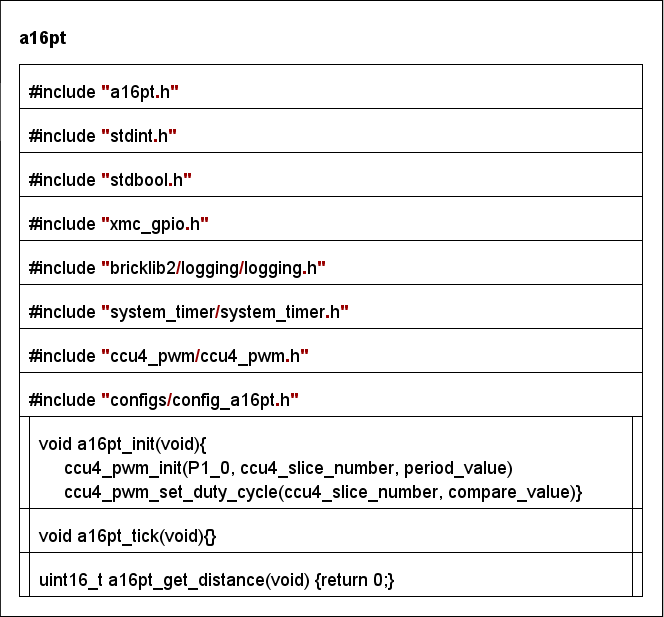
\includegraphics[width=1.0\textwidth]{Struktogramme/a16pt.png}\caption{Struktogramm der a16.pt}\label{fig:Bild2}
%\end{figure}
In der a16pt werden die für die Entfernungsmessung notwendigen Funktionen und die Interrupt anweisungen abgearbeitet, außerdem werden die Ein- und Ausgangsports hier geschaltet.\\

\chapter{Messungen und Auswertung der Ergebnisse}

Zu Beginn wurden Messungen direkt an dem Prozessor durchgeführt, um zu kontrollieren, dass die im Programm errechneten Signale auch die vorgesehenen Frequenzen erreichen. Anschließend wurden einzelne Baugruppen mit dem Prozessor kombiniert, um das Zusammenspiel dieser auswerten zu können. Danach wurden die Baugruppen um den Sensor erweitert und auch dieses Zusammenspiel wurde ausgewertet. Zum Abschluss wurde dann die komplette Platine im Betrieb getestet und optimiert.

\section{PWM-Ausgabe}
Um das Signal für die Entfernungsmessung zu generieren wurde der Mikrocontroller so programmiert, dass zehn Impulse mit einer Frequenz von 40kHz ausgegeben werden. Danach erfolgt eine Pause, um das zurückkehrende Signal abzuwarten und auszuwerten.\\
\begin{figure}[H]
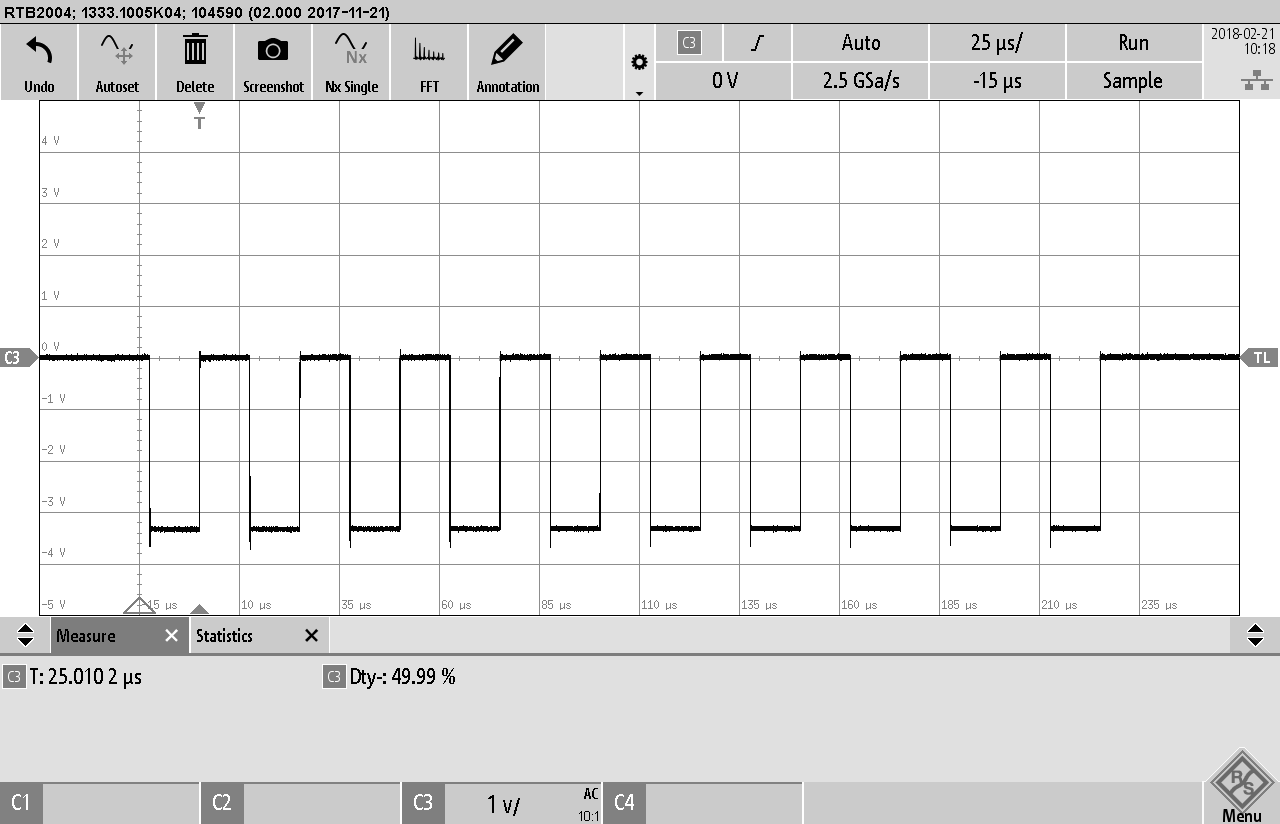
\includegraphics[width=1.0\textwidth]{Abbildungen/PWM-Signal.png}\caption{PWM-Burst auf 40kHz Basis}\label{fig:pwm-burst}
\end{figure}
In der Abbildung \ref{fig:pwm-burst} ist zu sehen, dass ein Burst aus zehn Impulsen mit einer Periodendauer von jeweils 25us generiert wurde. Diese Messung wurde direkt an dem Mikrocontroller vorgenommen, um sicherzustellen dass die H-Brücke mit der passenden Frequenz angesteuert wird.
\begin{figure}[H]
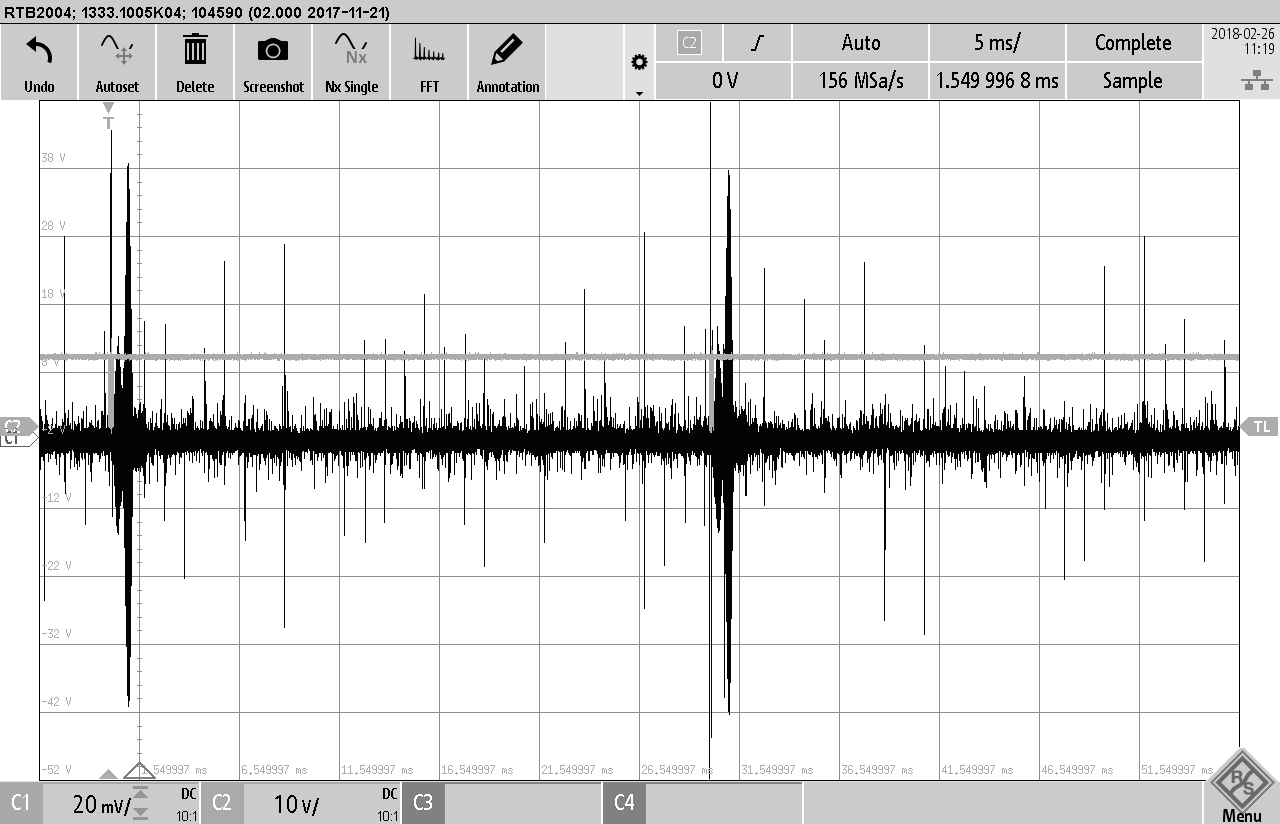
\includegraphics[width=1.0\textwidth]{Abbildungen/Abstand1.png}\caption{Versuchsmessung mit Sender und Empfänger parallel}\label{fig:Abstand1}
\end{figure}
In der Abbildung \ref{Abstand1} ist zu sehen, wie das Eingangssignal am Empfänger aussieht, wenn der Sender und der Empfänger getrennt aufgebaut sind und parallel auf ein Hinderniss gerichtet sind. Dabei zeigt die graue Linie den Verlauf des Sendersignals und die schwarze Linie den Verlauf des Empfängersignals
\section{H-Brücke}
Mach ersten Versuchen wurde die H-Brücke durch einen IXDN602, einen MOSFET ersetzt. Dies geschah, weil erstens die Beschaltung des OPV nur für eine positive Halbwelle funktioniert und zweitens die Beschaltung der H-Brücke fehlerhaft war. So wurde einer der Ausgänge auf Masse gelegt, was im Betrieb einen Kurzschluss verursachen würde. Um diese Probleme zu beheben, müssten der Sender- und der Empfängerkreis aufgetrennt werden und eine zweite Ultrashallkapsel eingesetzt werden. Dadurch ließ sich eine Reihe an Tests an der Senderschaltung durchführen. Allerdings viel auf, dass im Betrieb keine Signale empfangen wurden. Der Grund dafür war, dass der Mosfet als Low-Side-Driver geschaltet war, was bedeutet dass er das Signal entweder auf High, oder auf Low zieht. Somit werden auch alle von der Ultraschallkapsel empfangenen Signale direkt auf Low gezogen. Also musste eine weitere Überlegung angestellt werden und es wurden aus einem Mosfet zwei. Einer, der vom Prozessor angesteuert wird(3.3V) und den zweiten, der die Sendespannung(5V-20V) freigibt, schaltet. 

\section{Signalverlauf nach Verstärkung durch den OPV}
Durch die Verbindung der Sender- und der Empfängerseite entstand das Problem, dass die Entstörkondensatoren am Empfänger durch den Sendebetrieb zu sehr aufgeladen wurden, und sich danach erstmal entladen mussten, was eine Spannung am Sender/Empfänger zur Folge hatte. Das Entladen der Kondensatoren dauerte länger als die Pausen zwischen den Sendeimpulsen, dadurch konnten keine Signale empfangen werden.Um dieses Problem zu beheben wurde versucht, die OPV's durch einen MOSFET vom Sensor zu trennen, so lange gesendet wird. Da dieses erfolglos blieb wurde der Empfänger durch eine weitere Filterstufe erweitert.

\chapter{Ergebnisse der Forschung}
%Die Verwendung der H-Brücke war eine Fehlentscheidung, diese wurde durch einen MOSFET ersetzt. Das Problem mit der H-Brücke bestand darin, dass das gewählte Bauteil zum einen nicht zwangsläufig die gewünschte Schaltfrequenz halten kann.

\chapter{Fazit aus den Ergebnissen für denAuftraggeber}
%\input{9_Fazit_Auftraggeber}
\chapter{Reflektion über den Projektablauf}
\input{10_Reflektion_Ablauf}
\chapter{Anhänge}
\section{Schaltpläne}

\section{Platinenlayout}

\section{Quellcode}
Hier könnte Ihr Quellcode (inklusive Werbung) stehen\\
%\begin{lstlisting}
/* distance-us-v2-bricklet*/
/* Copyright (C) 2018 Olaf Lüke <olaf@tinkerforge.com>*/

/* a16pt.c: Driver for HDC1080 humidity sensor*/
*
* This library is free software; you can redistribute it and/or
* modify it under the terms of the GNU Lesser General Public
* License as published by the Free Software Foundation; either
* version 2 of the License, or (at your option) any later version.
*
* This library is distributed in the hope that it will be useful,
* but WITHOUT ANY WARRANTY; without even the implied warranty of
* MERCHANTABILITY or FITNESS FOR A PARTICULAR PURPOSE. See the GNU
* Lesser General Public License for more details.
*
* You should have received a copy of the GNU Lesser General Public
* License along with this library; if not, write to the
* Free Software Foundation, Inc., 59 Temple Place - Suite 330,
* Boston, MA 02111-1307, USA.
*/

#include "a16pt.h"
#include <stdint.h>
#include <stdbool.h>
#include <string.h>
/*********Infineon_eigene_Include_Datein*************/
#include "xmc_gpio.h"
#include "xmc_scu.h"
#include "xmc1_ccu4_map.h"
#include "xmc_ccu4.h"
/*************Eigene_Include_Dateien****************/
#include "bricklib2/logging/logging.h"
#include "system_timer/system_timer.h"
#include "eru/eru.h"
#include "ccu4_pwm_timer/ccu4_pwm_timer.h"
#include "configs/config_a16pt.h"
int x=0;int z=0;
uint32_t v=0; uint32_t v1=0;
int zeit=0; int zeit1=0;
/*************Interrupt_FUnktionen****************/
void IRQ_Hdlr_8(void)
{
	XMC_CCU4_SLICE_StopTimer(CCU40_CC40);
}
void IRQ_Hdlr_16(void)         //TIMER Überlauf Interrupt
{
	//XMC_GPIO_ToggleOutput(P0_0);
}
void IRQ_Hdlr_3(void) //ERU
{
	/*x=0;
	XMC_CCU4_SLICE_StartTimer(CCU40_CC40); */
}
void IRQ_Hdlr_7(void) 												// Compare Interrupt
{
}
void a16pt_init(void) {
//int messwerte[10]={};
/*****************Externe_Interrupt*******************/
	eru_init(eru_port);
/************PWM_Init********************************/
	ccu4_pwm_init(pwm_port, cc40, period_);
	ccu4_pwm_set_duty_cycle(cc40, compare_);
/************Event_Config****************************/
	count_init(cc41);
	capture_init(cc43);
/*******************Timer_2_Init*******************/
	ccu4_timer_2_init(cc42);
	XMC_CCU4_SLICE_StartTimer(CCU40_CC42);
	/*
	XMC_CCU4_SLICE_StopTimer(CCU40_CC42);
	XMC_CCU4_SLICE_ClearTimer(CCU40_CC42);
	*/
/********************LED_INIT*********************/
pin_out_init(P2_0);
pin_out_init(P0_0);
XMC_GPIO_SetOutputHigh(P2_0);
XMC_GPIO_SetOutputHigh(P0_0);
/**************Taster_INIT**********************/
pin_in_pullup_init(pullup_port);
}
void a16pt_tick(void) {
	static uint32_t debug_time = 0;
	static uint32_t signal_time = 0;
	// Print every 250ms
	if(system_timer_is_time_elapsed_ms(debug_time, 250)) {
		debug_time = system_timer_get_ms();
		uint32_t slice0 = XMC_CCU4_SLICE_GetTimerValue(CCU40_CC40);
		uint32_t slice1 = XMC_CCU4_SLICE_GetTimerValue(CCU40_CC41);
		uint32_t slice2 = XMC_CCU4_SLICE_GetTimerValue(CCU40_CC42);
		uint32_t slice3 = XMC_CCU4_SLICE_GetTimerValue(CCU40_CC43);
		logd("CCU40 s0: %d, s1: %d, s2: %d, s3: %d\n\r", slice0, slice1, slice2, slice3);
	}
	if(system_timer_is_time_elapsed_ms(signal_time, 33)) {
		signal_time = system_timer_get_ms();
		XMC_CCU4_SLICE_ClearTimer(CCU40_CC41);
		XMC_CCU4_SLICE_StartTimer(CCU40_CC40);
	}
	/*
	v1=XMC_CCU4_SLICE_GetTimerValue(CCU40_CC42);
	logd("v1:%d\n\r",v1);
if(XMC_GPIO_GetInput(P2_5)==0)
void a16pt_tick(void)
{
	for(z=0;z<messwerte[z];z++)
	{
		messwerte[z]=v1;
	}
}
if(v>1)
{
	zeit=(v/46.875)*4;
	logd("zeit:%d\n\r",zeit);
	zeit1=(v1/46.875)*4;
	logd("zeit1:%d\n\r",zeit1);
	XMC_CCU4_SLICE_ClearTimer(CCU40_CC42);
	v=0;
}
*/
}
uint16_t a16pt_get_distance(void)
{
return 0;
}
\end{lstlisting}



weitere Abbildungen
\listoffigures
\listoftables


\end{document}


